\chapter{Fundamentação Teórica}

A Fluidização é uma operação unitária baseada no escoamento ascendente (de baixo para cima) de um fluido, sendo este um líquido ou um gás, através de um leito de partículas sólidas granulares não consolidadas e não confinadas. Existe uma faixa estreita de velocidade desse fluido, abaixo da qual o leito é fixo e acima da qual é fluidizado, isto é, tem um comportamento semelhante ao de um fluido. No leito fixo, as partículas ocupam sempre as mesmas posições em relação ao vaso que contém o leito; e no leito fluidizado, as partículas se movem através dele. De fato, existe um limite superior de velocidade do fluido, acima do qual as partículas serão arrastadas do leito. Assim, quando se deseja promover o contato entre partículas sólidas e um fluido, uma das alternativas é fluidizar as partículas com o fluido.


Para entender o fenômeno da fluidização, considere uma massa de partículas acomodada sobre uma placa ou tela perfurada, formando um leito de seção transversal circular ou retangular. Agora imagine uma corrente gasosa atravessando esse leito de partículas no sentido ascendente, como se mostra a Figura \ref{fig1}.


\begin{figure}[H]
	\begin{center}
		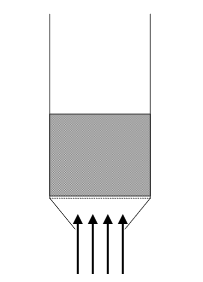
\includegraphics[scale=.8, trim={0 0 0 0}]{figuras/ladeq/fluid/fig1}
		%\vspace{-20pt}
		\caption{Leito de partículas percolado por uma corrente gasosa ascendente.}
		\label{fig1}
	\end{center}
\end{figure}


Com uma baixa velocidade do gás, este escoa nos espaços entre as partículas, sem promover movimentação do material — o qual caracteriza-se por uma simples percolação, onde o leito permanece fixo. À medida que se aumenta a velocidade do gás, as partículas se afastam e algumas começam a apresentar uma leve vibração — tem-se nesse momento um leito expandido.

Com velocidade ainda maior, atinge-se uma condição em que a soma das forças de fricção entre as partículas e o fluido, causadas pelo escoamento do gás no sentido ascendente iguala-se ao peso das partículas. Nessa situação, em que o movimento do material é mais vigoroso, atinge-se o que se chama de leito fluidizado. À velocidade do gás nessa condição dá-se o nome de mínima velocidade de fluidização, que é a velocidade correspondente ao regime de fluidização incipiente.

Continuando-se o processo de aumento da velocidade do gás, a fluidização borbulhante é o regime que se observa após a fluidização incipiente. No caso de partículas de pequeno tamanho, com densidade geralmente menor do que $ 1,4 \ \dfrac{g}{cm^{3}} $, ocorre uma expansão considerável do leito antes de surgirem as bolhas que caracterizam a fluidização borbulhante. No caso de partículas mais densas, entre $ 1,4 \ \dfrac{g}{cm^{3}} $ e $ 4 \ \dfrac{g}{cm^{3}} $, a expansão do leito não vai muito além daquela adquirida na condição de fluidização incipiente e as bolhas já surgem com a velocidade mínima de fluidização.

O regime seguinte ao turbulento é o de fluidização rápida, que acontece quando a velocidade do gás excede a velocidade terminal de sedimentação das partículas e o material passa a ser arrastado. Com velocidades ainda maiores, suficientes para arrastar todo o material, atinge-se a condição de transporte pneumático. Para operar o sistema nessas condições deve haver uma operação subsequente de separação gás-sólido. Na Figura \ref{fig2} mostram-se os tipos de regime de fluidização em função da velocidade do gás e sua queda de pressão ao escoar através do leito de partículas.

\begin{figure}[H]
	\begin{center}
		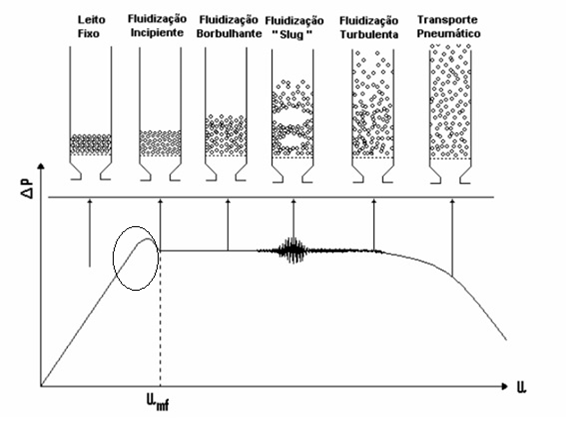
\includegraphics[scale=.8, trim={0 0 0 0}]{figuras/ladeq/fluid/fig2}
		%\vspace{-20pt}
		\caption{Regimes de fluidização em função da velocidade superficial do gás.}
		\label{fig2}
	\end{center}
\end{figure}

\begin{figure}[H]
	\begin{center}
		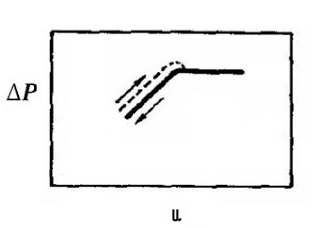
\includegraphics[scale=.8, trim={0 0 0 0}]{figuras/ladeq/fluid/fig3}
		%\vspace{-20pt}
		\caption{Fluidização x Desfluidização – Fenômeno de Histerese.}
		\label{fig3}
	\end{center}
\end{figure}


Após a realização da fluidização, existe a etapa de desfluidização, o qual ocorre em sentido e de forma contrária à primeira, ou seja, o controle da vazão de ar diminui proporcionalmente às vazões escolhidas na etapa de fluidização, até que se atinja a vazão zero. È interessante observar que a curva de desfluidização no gráfico (linha cheia da Figura 3) não coincide com a curva de fluidização, tal fenômeno é conhecido como Histerese. Isso ocorre porque, no momento em que o leito é desfluidizado após o escoamento de ar, sua porosidade muda e as partículas sólidas não voltam ao estado de compactação anterior a tempo.

A eficiência da fluidização depende da velocidade de ascensão do fluido, da sua viscosidade e densidade, bem como da distribuição de tamanhos do sólido, de sua densidade, da porosidade do leito e da seção transversal do leito.

Por possuir vantagens como, por exemplo, promover elevados coeficientes de transferência de calor e de massa entre o fluido e o sólido e também entre as partículas do sólido, ao realizar uma mistura rápida (o que proporciona uma distribuição isotérmica  de temperaturas entre o leito); facilitar um controle automático, por ter um comportamento semelhante a um líquido; e possuir uma elevada superfície de contato, os leitos fluidizados integram processos de produção em inúmeras áreas da engenharia química, tanto em processos químicos quanto em processos físicos. Na indústria química e petroquímica são empregados no coqueamento e produção de alumínio, no cracking catalítico para produção de gasolina, cracking térmico para produzir etileno e propileno, além de servir ainda para a polimerização deste último. Em processos físicos, é possível verificar o uso de fluidização para aquecimento, secagem, elutriação, transporte de sólidos e mistura de pós finos, em que na indústria alimentícia os leitos fluidizados participam dos sistemas de torrefação de café, congelamento e secagem de alimentos e ainda no recobrimento de doces e pastilhas e sistemas de microencapsulação.

A engenharia química já desenvolveu diversas aplicações para a fluidização, em especial no tocante aos reatores químicos e secadores. Há ainda algumas desvantagens que comprometem o bom desempenho da fluidização, como a ocorrência de erosão do equipamento em razão do frequente impacto dos sólidos e o consumo de energia devido à alta perda de carga requerendo, portanto, alta velocidade do fluido.


\chapter{Objetivos}

O objetivo principal da prática foi realizar a fluidização da areia a partir da passagem de uma vazão de gás ascendente sobre o leito. Além disso, outras etapas foram requeridas:

\begin{itemize}
	\item Determinar a massa específica das partículas de areia e da água.
	\item Construir o gráfico (log-log) de queda de pressão versus velocidade superficial do ar.
	\item Construir o gráfico (log-log) da altura do leito versus velocidade superficial do ar.
	\item Determinar experimentalmente as condições mínimas de fluidização: $\left(\varepsilon_{\mathrm{mf}}\right)$; $ u_{mf} $; $ L_{mf} $.
	\item Determinar a queda de pressão teórica $ (\Delta Pf) $ e comparar com valor experimental.
	\item Determinar a porosidade mínima de fluidização teórica $\left(\varepsilon_{\mathrm{mf}}\right)$ e comparar com o valor experimental.
	\item Determinar a velocidade superficial mínima de fluidização teórica $ (u_{mf}) $ pelas correlações de Miller e Logwinug; Leva; Davies e Richardson e comparar com o valor experimental.
	\item Calcular, com base nos dados experimentais, a permeabilidade k do leito fixo antes (compactado) e depois de fluidizar o leito. Fazer uma análise crítica dos dois valores.
	\item Estimar a esfericidade média $ (\Phi) $ da areia com os dois valores de k obtidos no item anterior por meio da correlação de Kozeny-Cármán.
\end{itemize}


\chapter{Materiais}

\begin{itemize}
\item Areia;
\item Ar;
\item Água destilada;
\item Picnômetro;
\item Balança;
\item Tubo (coluna) de vidro vertical (local de depósito da areia);
\item Suporte para o tubo (coluna) de vidro vertical;
\item Régua;
\item Vazão de gás proveniente da tubulação;
\item Tubo Pitot de medição do $ \Delta P $ (tubo em U preenchido com líquido); e
\item Mangueiras para conectar os equipamentos.

\end{itemize}


\chapter{Descrição da Unidade}


\begin{figure}[H]
	\begin{center}
		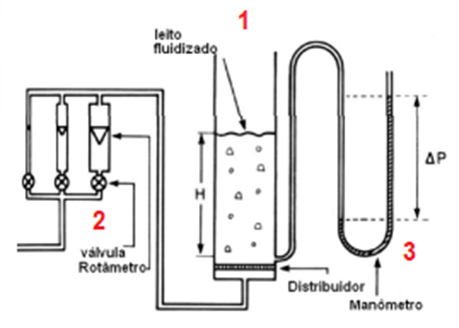
\includegraphics[scale=.8, trim={0 0 0 0}]{figuras/ladeq/fluid/fig4}
		%\vspace{-20pt}
		\caption{ Esquema do equipamento usado para a Fluidização.}
		\label{fig4}
	\end{center}
\end{figure}

onde:

\begin{itemize}
\item "1": Tubo (coluna) de vidro vertical contendo as partículas de areia e por onde passa o fluxo de ar;
\item "2": Válvula de Controle para a vazão de ar; e
\item "3": Tubo Pitot contendo um líquido para medir a queda da pressão $ (\Delta P) $.
\end{itemize}


\chapter{Metodologia Teórica e Experimental}

\section{Picnometria}


A densidade média das partículas de areia pode ser obtida através do método da Picnometria. Tal metodologia é amplamente utilizada para a determinação da massa específica e da densidade de diversas substâncias.

A técnica é baseada na utilização de um picnômetro, uma vidraria especial esmerilhada que possui um baixo coeficiente de dilatação, e diversas pesagens envolvendo o picnômetro, a areia (analito em questão) e água (líquido padrão).As massas pesadas são:

\begin{figure}[H]
	\begin{center}
		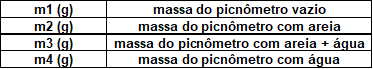
\includegraphics[scale=.8, trim={0 0 0 0}]{figuras/ladeq/fluid/fig5}
		%\vspace{-20pt}
		\label{fig5}
	\end{center}
\end{figure}

De posse das massas, é calculada a densidade relativa da areia (SGs):

\begin{equation}\label{key}
\mathrm{SG}_{\mathrm{S}}=\frac{\mathrm{m}_{2}-\mathrm{m}_{1}}{\left(\mathrm{m}_{4}-\mathrm{m}_{1}\right)-\left(\mathrm{m}_{3}-\mathrm{m}_{2}\right)}
\end{equation}


Então, com o valor da massa específica da água na temperatura do experimento, é calculada a massa específica da areia usando a equação:

\begin{equation}\label{key}
\rho_{\mathrm{S}}=\mathrm{SG}_{\mathrm{S}} \rho_{\mathrm{água}}
\end{equation}



\begin{itemize}
\item Determinar o diâmetro interno do tubo de vidro que irá conter o leito fluidizado; 

Antes de começar o experimento de fluidização, mediu-se, com o auxílio de uma régua, o diâmetro interno do tubo (coluna) de vidro para a realização dos cálculos posteriores:

$\mathrm{d}_{\text { interno do tubo }}=4,4 \ \mathrm{cm}$

\item Pesar uma massa de areia de no mínimo 300g e transferi-la para o tubo de vidro;

$\mathrm{m}_{\mathrm{areia}}=305,57 \ \mathrm{g}$

\item Após a pesagem, retirou-se o tubo de vidro do suporte e transferiu-se a areia para o seu interior. 

\item Após a pesagem, retirou-se o tubo de vidro do suporte e transferiu-se a areia para o seu interior. 

Antes de abrir a válvula de vazão de ar, mediu-se a altura inicial do leito e verificou-se a diferença de pressão $ (\Delta P) $ sendo zero.

$\mathrm{L}_{\mathrm{leito}}=9,5 \ \mathrm{cm}$

\item Abrir vagarosamente a válvula de controle de ar de modo a obter uma vazão baixa e constante através do leito;

O primeiro valor de vazão de ar foi de 2 L/min e, em seguida, a vazão seria aumentada a cada 1 L/min para que os novos valores de altura do leito e de pressão $ P_{1} $ e $P_{2}$ fossem anotados.

\item Anotar a vazão de ar indicada pelo rotâmetro;

\item Anotar a correspondente queda de pressão (coluna de água) no tubo em U;

\item Verificar se houve variação na altura do leito de partículas e anotar;

\item Aumentar a vazão de ar através do sistema abrindo um pouco mais a válvula;


\item Repetir as últimas 5 etapas até que se obtenha um leito plenamente fluidizado com a presença de bolhas de ar. Vazões muito altas podem causar arraste de partículas, diminuindo a massa do leito;

vazão máxima de Fluidização alcançada: Q = 10 L/min


\item Fechar vagarosamente a válvula de modo a diminuir a vazão de ar;

Nessa etapa começou-se o processo de Desfluidização, semelhante à Fluidização, porém em etapa reversa de vazão, em que esta foi diminuída a cada 1 L/min até atingir o ponto zero.

\item Anotar a vazão indicada pelo rotâmetro;

\item Anotar a correspondente queda de pressão (coluna de água) no tubo em U;

\item Verificar se houve variação na altura do leito de partículas e anotar; e

\item Repetir as últimas 4 etapas até que se atinja a vazão de ar que se iniciou o experimento.
\end{itemize}

\chapter{Resultados e Discussão}

\section{Massa específica da areia}

Os resultados das pesagens para a picnometria foram:

\begin{table}[H]
	\centering
	\begin{tabular}{|c|c|c|}
		\hline
		m1 (g) & 36,4606 & massa do picnômetro vazio            \\ \hline
		m2 (g) & 53,1301 & massa do picnômetro com areia        \\ \hline
		m3 (g) & 71,3707 & massa do picnômetro com areia + água \\ \hline
		m4 (g) & 60,9335 & massa do picnômetro com água         \\ \hline
		T °C   & 25      & Temperatura Ambiente                 \\ \hline
	\end{tabular}
	\caption{Dados da picnometria.}
	\label{table1}
\end{table}

De posse das massas, foi calculada a densidade relativa da areia (SGs) e, com o valor da massa específica da água a $ 25 \ ^{\circ}C $, a massa específica da areia usando:


\begin{figure}[H]
	\begin{center}
		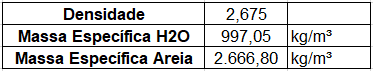
\includegraphics[scale=1, trim={0 0 0 0}]{figuras/ladeq/fluid/fig6}
		%\vspace{-20pt}
		\label{fig6}
	\end{center}
\end{figure}

\section{Fluidização}

Os resultados de diferença de pressão, altura e vazão do experimento são mostrados na Tabela da Figura \ref{fig12}:

\begin{figure}[H]
	\begin{center}
		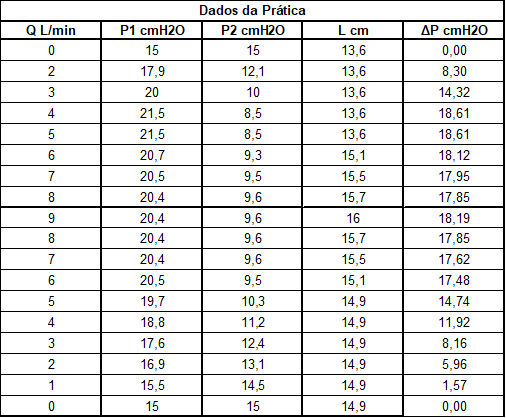
\includegraphics[scale=1, trim={0 0 0 0}]{figuras/ladeq/fluid/fig7}
		%\vspace{-20pt}
		\label{fig12}
		\caption{Resultados obtidos no experimento de Fluidização-Desfluidização}
	\end{center}
\end{figure}

Com eles, foram traçados os gráficos log-log da queda de pressão e da altura do leito versus a vazão de ar:


\begin{figure}[H]
	\begin{center}
		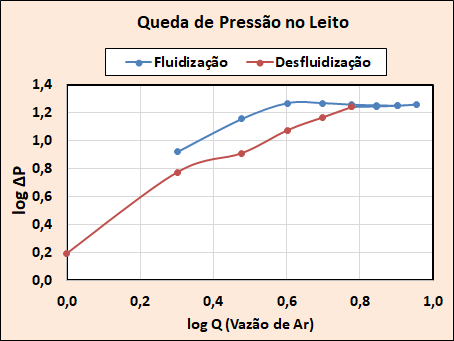
\includegraphics[scale=1, trim={0 0 0 0}]{figuras/ladeq/fluid/graph1}
		%\vspace{-20pt}
		\label{fig7}
		\caption{Gráfico (log-log) de queda de pressão do leito versus vazão de ar.}
	\end{center}
\end{figure}


\begin{figure}[H]
	\begin{center}
		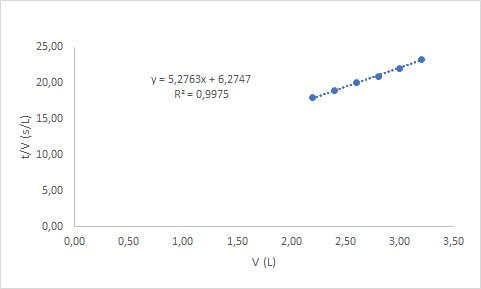
\includegraphics[scale=1, trim={0 0 0 0}]{figuras/ladeq/fluid/graph2}
		%\vspace{-20pt}
		\label{fig7}
		\caption{Gráfico (log-log) da altura de leito poroso versus vazão de ar.}
	\end{center}
\end{figure}


Com o gráfico de queda de pressão, foi determinado experimentalmente a vazão mínima de fluidização:


\begin{figure}[H]
	\begin{center}
		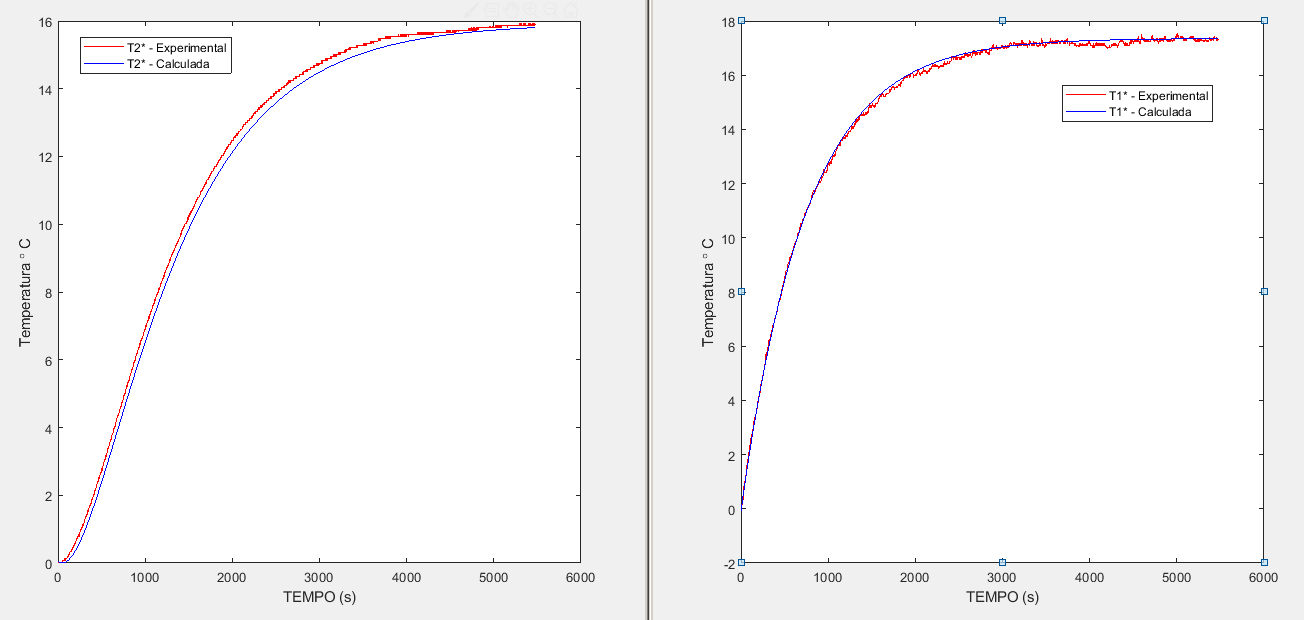
\includegraphics[scale=1, trim={0 0 0 0}]{figuras/ladeq/fluid/graph3}
		%\vspace{-20pt}
		\label{fig7}
		\caption{Gráfico (log-log) de queda de pressão do leito versus vazão de ar.}
	\end{center}
\end{figure}

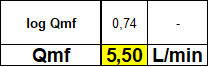
\includegraphics[scale=.8, trim={0 0 0 0}]{figuras/ladeq/fluid/table1}

Gráfico (log-log) de queda de pressão do leito versus vazão de ar

\begin{equation}\label{key}
u_{m f}=\frac{Q_{m f}}{S}
\end{equation}


Sendo a área transversal:$  S=0,001521 \ m^2 $


\begin{equation}\label{key}
u_{m f}=0,0603 \frac{m}{s}
\end{equation}


Com este valor, é calculado, utilizando o gráfico de altura do leito, a altura de leito mínima Hmf:

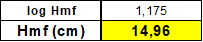
\includegraphics[scale=.8, trim={0 0 0 0}]{figuras/ladeq/fluid/table2}

Com a altura mínima e os dados do aparato, foi calculada a porosidade mínima de fluidização:


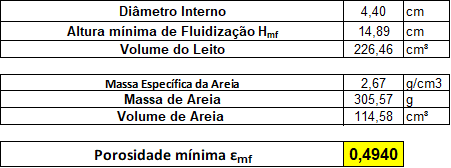
\includegraphics[scale=1, trim={0 0 0 0}]{figuras/ladeq/fluid/table3}


\chapter{Cálculos}


\section{Determinação da Queda de Pressão Teórica}

É observado experimentalmente que a queda de pressão no leito fluidizado é aproximadamente igual ao peso do leito (sólido e fluido). 

Como a baixas pressões a densidade dos sólidos é 3 vezes maior que a densidade de gases, o peso do leito pode ser considerado igual ao peso dos sólidos e a queda de pressão pode ser estimada por:

\begin{equation}\label{key}
\Delta \mathrm{p} \cong \frac{\text { peso do solido }}{\text { área transversal }} (\text{leitos fluidizados a gás})
\end{equation}

Calculando o peso com a massa de areia e a área com o diâmetro interno do tubo, tem-se:

\begin{equation}\label{key}
\Delta P_{\text {teorica}}=\dfrac{\operatorname{Massa} _{\text {areia}} \times g}{\dfrac{\pi d^{2}}{4}}
\end{equation}

Por essa equação, a queda de pressão teórica calculada é de $ 20,16 \ cmH_{2}O $.

O valor obtido experimentalmente foi em torno de $ 18 \ cmH_{2}O $, o que dá uma diferença de 11\%.

\section{Determinação da Porosidade Mínima de Fluidização Teórica}

Podemos determinar também a porosidade mínima de fluidização teórica. Para isso, partimos da relação de igualdade entre a força de pressão do fluido $ (F_P) $ e a força peso do leito $ (F_g) $, pois é nessa condição que o leito começará a fluidizar.

\begin{equation}\label{key}
\left(F_{p}\right)=\left(F_{g}\right)
\end{equation}

Definindo cada lado da equação:

\begin{equation}\label{key}
\left(F_{P}\right)=(-\Delta P) \cdot S
\end{equation}

\begin{equation}\label{key}
\left(F_{g}\right)=\left(\rho_{p}-\rho_{f}\right) \cdot S \cdot L \cdot(1-\varepsilon) \cdot g
\end{equation}

Igualando-os:

\begin{equation}\label{key}
(-\Delta P) \cdot S=\left(\rho_{p}-\rho_{f}\right) \cdot S \cdot L \cdot(1-\varepsilon) \cdot g
\end{equation}

\begin{equation}\label{key}
\frac{(-\Delta P)}{L}=\left(\rho_{p}-\rho_{f}\right) \cdot(1-\varepsilon) \cdot g
\end{equation}


Onde:

\begin{itemize}
\item $ \rho_f $: massa específica do ar;
\item $ \rho_p $: massa específica da areia;
\item S: seção transversal do leito.
\end{itemize}

\newpage

Considerando $ \rho_f $ desprezível frente a $ \rho_p $, temos:

\begin{equation}\label{key}
\frac{-\Delta P_{f}}{L_{m f}}=\rho_{\text {areia}} \cdot\left(1-\varepsilon_{m f}\right) \cdot g
\end{equation}

Sabendo que:

\begin{equation}\label{key}
\Delta P_{f, \text{teórico}}=20,16 \ \mathrm{cm} \mathrm{H_{2}O} = 19769,7 \ \frac{g}{s^{2} \cdot \mathrm{cm}}
\end{equation}

\begin{equation}\label{key}
\varepsilon_{m f}=1+\left(\frac{\Delta P_{f}}{L_{m f}} \cdot \frac{1}{\rho_{\text {areia}} \cdot g}\right)=1+\left(\frac{19769,7}{14,89} \cdot \frac{1}{2,67 \cdot 981}\right)
\end{equation}

\begin{equation}\label{key}
\varepsilon_{m f}=0,4931
\end{equation}

Comparando com o valor experimental que foi de 0,4940, chegamos a um erro percentual de apenas 0,18\%. Isso indica que o comportamento da prática foi condizente com a teoria.

\section{Determinação da Velocidade Mínima de Fluidização Teórica}

Faremos o cálculo teórico a partir de 3 correlações conhecidas.

\subsection{Miller e Logwinug}


\begin{equation}\label{key}
G_{m f}=0,00125 \dfrac{d^{2} \cdot\left(\rho_{s}-\rho\right)^{0.9} \cdot \rho^{1,1} \cdot g}{\mu}
\end{equation}

\begin{equation}\label{key}
G_{m f}=0,0514 \frac{k g}{m^{2} \cdot s}
\end{equation}

Sabendo que:

\begin{equation}\label{key}
G_{m f}=u_{m f} \cdot \rho
\end{equation}

Temos:

\begin{equation}\label{key}
u_{m f}=0,0432 \ \frac{m}{s}
\end{equation}



\subsection{Leva}

\begin{equation}\label{key}
G_{m f}=0,0093 \frac{d^{1.82} \cdot\left(\rho\left(\rho_{s}-\rho\right)\right)^{0.94}}{\mu^{0.88}}
\end{equation}

\begin{equation}\label{key}
G_{m f}=0,0635 \ \dfrac{k g}{m^{2} \cdot s}
\end{equation}

Analogamente:

\begin{equation}\label{key}
u_{m f}=0,0534 \ \frac{m}{s}
\end{equation}

\subsection{Davies e Richardson}


\begin{equation}\label{key}
G_{m f}=0,0078 \dfrac{d^{2} \cdot \rho\left(\rho_{s}-\rho\right)^{2} \cdot g}{\mu}
\end{equation}

\begin{equation}\label{key}
G_{m f}=0,0694 \ \dfrac{k g}{m^{2} \cdot s}
\end{equation}

\begin{table}[H]
	\centering
	\begin{tabular}{|c|c|}
		\hline
		\textbf{Modelo}     & \textbf{umf (m/s)} \\ \hline
		Miller e  Logwinug  & 0,0432             \\ \hline
		Leva                & 0,0534             \\ \hline
		Davies e Richardson & 0,0583             \\ \hline
		Experimental        & 0,0603             \\ \hline
	\end{tabular}
	\caption{Comparação entre os resultados obtidos para cada modelo.}
	\label{tabmodel}
\end{table}


Dos valores obtidos podemos concluir que o modelo de Davies e Richardson foi aquele que mais se aproximou do valor experimental, apresentando um erro de apenas 3,32\%.

\section{Determinação da Permeabilidade (K)}

Para a determinação da permeabilidade precisamos analisar o sistema antes e depois da fluidização quando ainda em estado de leito fixo. Para isso iremos utilizar a equação abaixo:


\begin{equation}\label{key}
\frac{\Delta P}{L \cdot q}=\frac{c \rho}{\sqrt{k}} q+\frac{\mu}{k}(1)
\end{equation}

Utilizando uma regressão linear onde:

\begin{itemize}
	\item $y=\frac{\Delta P}{L \cdot q}$;
	\item $x=q$;
	\item $b=\frac{\mu}{k}$.
\end{itemize}


Dados antes da fluidização:

\begin{figure}[H]
	\begin{center}
		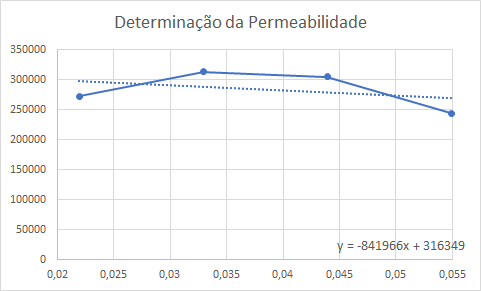
\includegraphics[scale=.8, trim={0 0 0 0}]{figuras/ladeq/fluid/graph4}
		%\vspace{-20pt}
		\label{fig7}
		\caption{Gráfico da equação (1) para o leito fixo antes da fluidização.}
	\end{center}
\end{figure}

Logo,

\begin{equation}\label{key}
b=\frac{\mu}{k}=316349 \frac{\mathrm{kg}}{\mathrm{m}^{2} \cdot \mathrm{s}}
\end{equation}

\begin{equation}\label{key}
k=\frac{\mu}{316349}=\frac{0,0000184}{316349}
\end{equation}

\begin{equation}\label{key}
k=5,82 \cdot 10^{-11} \ \mathrm{m}^{2}
\end{equation}

Dados depois da fluidização:

\begin{figure}[H]
	\begin{center}
		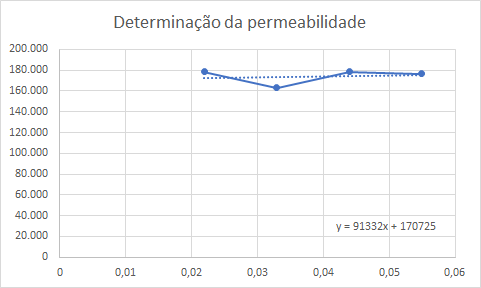
\includegraphics[scale=.8, trim={0 0 0 0}]{figuras/ladeq/fluid/graph5}
		%\vspace{-20pt}
		\label{fig7}
		\caption{Gráfico da equação (1) para o leito fixo depois da fluidização.}
	\end{center}
\end{figure}

Analogamente,

\begin{equation}\label{key}
b=\frac{\mu}{k}=901727 \frac{k g}{m^{2} \cdot s}
\end{equation}


\begin{equation}\label{key}
k=\frac{\mu}{316349}=\frac{0,0000184}{170725}
\end{equation}

\begin{equation}\label{key}
k=10,78 \cdot 10^{-11} \ m^{2}
\end{equation}

A partir desses dados calculados, notamos que há um aumento da permeabilidade comparando-se o leito fixo pré-fluidização e o leio fixo pós-fluidização. Isso é coerente, pois antes da fluidização o leito está mais compactado. Essa compactação resulta numa menor permeabilidade se comparado ao leito após a fluidização.

\section{Determinação da Esfericidade $ (\mathrm{\Phi}) $}

Com os valores de permeabilidades calculados acima, pôde-se então calcular a esfericidade das partículas com o modelo de Kozeny-Cárman, sabendo que a constante $ \beta $ é igual a 5,0 para meios porosos granulares. Assim, tem-se:

\begin{equation}\label{key}
k=\frac{\left(\Phi \times d_{p}\right)^{2} \times \varepsilon^{3}}{36 \times \beta \times(1-\varepsilon)^{2}}
\end{equation}

\begin{equation}\label{key}
\not \vec{p}=\sqrt{\frac{36 \beta(1-\varepsilon)^{2} k}{d_{p}^{2} \varepsilon^{s}}}
\end{equation}

Onde antes da fluidização:


\begin{itemize}
\item k é a permeabilidade do meio = $ 5,82 \times 10^{-11} m^{2} $;
\item $ \mathrm{\Phi} $ é a esfericidade média da partícula;
\item $ d_p $ é o diâmetro médio da partícula = 0,0002293 m;
\item $ \varepsilon $ é a porosidade = 0,4940 (achada experimentalmente);
\item $ \beta $ é um parâmetro do modelo que depende do meio = 5,0.
\end{itemize}


\begin{equation}\label{key}
\Phi=\sqrt{\frac{36 \times 5,0 \times(1-0,4940)^{2} \times\left(5,82 \times 10^{-11} m^{2}\right)}{(0,0002293 m)^{2} \times(0,4940)^{s}}}
\end{equation}

\begin{equation}\label{key}
\Phi=0,6505
\end{equation}

E depois da fluidização:

\begin{itemize}
\item k é a permeabilidade do meio $ = 10,78 \cdot 10^{-11} \ m^{2} $;
\item $ \mathrm{\Phi} $ é a esfericidade média da partícula;
\item $ d_p $ é o diâmetro médio da partícula = 0,0002293 m;
\item $ \varepsilon $ é a porosidade = 0,4940 (achada experimentalmente);
\item $ \beta $ é um parâmetro do modelo que depende do meio = 5,0.
\end{itemize}

\begin{equation}\label{key}
\Phi=\sqrt{\frac{36 \times 5,0 \times(1-0,4940)^{2} \times\left(10,78 \cdot 10^{-11} m^{2}\right)}{(0,0002293 m)^{2} \times(0,4940)^{s}}}
\end{equation}

\begin{equation}\label{key}
\Phi=0,8853
\end{equation}

Em que a média entre os valores das esfericidades de antes e de depois da Fluidização é: 

\begin{equation}\label{key}
\Phi _{\text{média}}=\left(\frac{0,6505+0,8853}{2}\right)
\end{equation}

\begin{equation}\label{key}
\Phi _{\text{média}}=0,7679
\end{equation}

\chapter{Conclusão}

Os resultados experimentais foram satisfatórios analisando de uma forma geral visto que a maioria dos resultados ficou relativamente próxima de seus respectivos valores teóricos e que também corresponderam em grande parte às tendências esperadas.

Os gráficos gerados com o avanço da fluidização e desfluidização corresponderam às expectativas de comportamento ficando claro o efeito de histerese apresentado na introdução.

Para a determinação da queda de pressão teórica, tivemos um erro de 11\%. Que é um erro relevante, mas não chega a impedir a utilização do modelo nesse caso. Já para a porosidade mínima de fluidização o valor encontrado experimentalmente teve um erro desprezível e, portanto, foi muito coerente.

Para a velocidade mínima de fluidização e esfericidade não foi diferente. Foram encontrados valores de velocidade muito próximos do teórico e a esfericidade foi relativamente alta, como esperado para grãos de areia.


